\begin{savequote}[45mm]
Everything in nature is some field configuration.
\qauthor{Urs Schreiber}
\end{savequote}
\chapter{Field Theory}
\section{What is a field?}
 A field is some local function in space with some definite transformations under the symmetries we would like to introduce in the theory. A scalar field is function that spits out a scalar for every point in space=time. Note this scalar can be from $\mathbb{R}$ or $\mathbb{C}$.
\section{Lagrangians for Fields}
When we're talking about fields being elements of the Lagrangian, we need to integrate over all of the field $\phi$
\begin{equation}
    S = \int_{a}^{b} \mathcal{L}(\phi, \partial_{\mu} \phi, t) \ d^{4}x
\end{equation}
We can relate the "new curly" Lagrangian to the old one as follows:
\begin{equation}
   \int_{a}^{b} L dt = \int_{a}^{b} \mathcal{L}(\phi, \partial_{\mu} \phi, t) \ d^{3}x
\end{equation}
We call the new Lagrangian the \textbf{Lagrangian density}. Which also means we can define a momentum density
\begin{equation}
    \Pi = \frac{\partial \mathcal{L}}{\partial(\partial_{\mu} \phi)}
\end{equation}
Now the modified Euler-Lagrange equation reads
\begin{equation}
     \frac{\partial \mathcal{L}}{\partial \phi} - \partial_{\mu} \left( \frac{\partial \mathcal{L}}{\partial(\partial_{\mu} \phi)} \right) = 0
\end{equation}
Similarly we can define the Hamiltonian density as
\begin{equation}
    H = \int_{a}^{b} \ \mathcal{H} \ d^{3}x = \Pi \partial_{\mu} \phi - \mathcal{L}
\end{equation}
Combining all of this we can introduce the of Noether current
\begin{equation}
    j^{\mu} = p^{\mu}\xi - \mathcal{H}^{\mu}_{\rho}\tau^{\rho}
\end{equation}
whose continuity equation reads
\begin{equation}
    \partial_{\mu} j^{\mu} = 0
\end{equation}
\section{The Klein-Gordon Equation}
The Klein-Gordon equation essentially models spin-0 particles without any external potentials i.e. sources.
Let's derive it from what we've seen so far. We start by looking at plane wave solutions to the Schrodinger equation
\begin{equation}
    \phi(x,t) = Ne^{-i(\omega t -k.x)} = Ne^{-ip.x} 
\end{equation}
where $N$ is the normalization constant. We shall call a wave with such a sign combination an \textbf{incoming wave}. So what happens when we operate on it with the energy and momentum operators? We get the following
\begin{equation} \label{energop}
\hat{E}\phi(x,t) = i \hbar \frac{\partial}{\partial t}(Ne^{-i(\omega t -k.x)}) = \hbar \omega \phi(x,t)
\end{equation}

\begin{equation} \label{momenop}
\hat{P}\phi(x,t) = -i \hbar \nabla (Ne^{-i(\omega t -k.x)}) = \hbar k \phi(x,t)
\end{equation}
We have the relation
\begin{equation}
    E = {(p^{2}c^{2} + m^{2}c^{4})}^{1/2}
\end{equation}
Now let's substitute the terms with operators acting on $\phi$
\begin{equation}
    i \hbar \frac{\partial \phi(x,t)}{\partial t} = {(-\hbar^{2}c^{2}\nabla^{2} + m^{2}c^{4})}^{1/2}\phi(x,t)
\end{equation}
This at first glance does not seem covariant, so let's square it
\begin{equation}
    - \hbar^{2} \frac{\partial^{2} \phi(x,t)}{\partial t^{2}} = (-\hbar^{2}c^{2}\nabla^{2} + m^{2}c^{4}) \phi(x,t)
\end{equation}
By setting $\hbar = c = 1$ this can be succintly written as
\begin{equation}
    (\partial^{2} + m^{2}) \phi(x) = 0
\end{equation}
\subsection{Probability Currents}
Although it follows from what we know pretty straightforwardly, it wasn't taken very seriously for one specific reason, let's see why. From the continuity equation we have 
\begin{equation}
    \frac{\partial \rho}{\partial t} = - \nabla . J
\end{equation}
for the case of non-relativistic quantum mechanics, we have
\begin{equation}
    j(x)  = - i\left[ \phi^{*}(x) \nabla \phi - \phi \nabla \phi^{*}(x) \right]
\end{equation}
and for the probability density
\begin{equation}
    \rho(x) = i \left[ \phi^{*}(x) \frac{\partial \phi}{\partial t} - \phi \frac{\partial \phi^{*}(x)}{\partial t} \right]
\end{equation}
these can be combined and written covariantly as
\begin{equation}
    j^{\mu}(x) = i\left[ \phi^{*}(x) \partial_{\mu} \phi - [\partial_{\mu} \phi^{*}(x)]\phi \right]
\end{equation}
Substituting in our wavefunction $\phi(x) = Ne^{-p.x}$, we find that the time component is of the form
\begin{equation}
    j^{0} = \rho = 2{|N|}^{2}E
\end{equation}
Since $E$ can be positive or negative we can't interpret $\rho$ as a probability density as it is non-sensical to talk about negative probabilities. Or is it?
\subsection{A new Interpretation}
Fortunately, not all is lost. Richard Feynman and Ernst Stuckelberg came up with a unique interpretation independently. They suggested that we can view negative energy states as simply particles travelling back in time. What? 
This is because changing the sign of the proper time $\tau$ has the same effect as
changing the sign of the charge. Therefore, a particle travelling backward in time looks the same as an oppositely charged antiparticle moving forward in time. One strategy to eliminate negative energy states
is therefore to reverse the charge and momentum of all negative energy
solutions, turning them into antiparticles. How does this eliminate the
negative sign of the energy? Since we write the phase of the wave function as $Et − p · x$, then making the substitution $t \rightarrow −t$ means that we
have to change $−E \rightarrow E$ for the first term to make sense. Of course
reversing the time (like playing a film backwards) reverses all momenta
so we also need to swap $p \rightarrow −p$ for consistency
We  can visualize this as follows
\begin{figure}
	\centering
	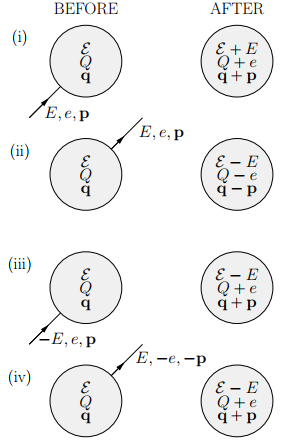
\includegraphics[scale=0.8]{Figures/parvis.png}
	\caption{ (i) An incoming particle (energy $E$, charge $e$ ($= |e|$), momentum
$p$) is absorbed by a system (energy $E$,
charge $Q$, momentum $q$). Also shown
are (ii) emission of particle, (iii) absorption of a particle in a negative energy
state and (iv) emission of an antiparticle in a positive energy state.}
\end{figure}
Thus simply put, a general solution to the Klein-Gordon equation is of the form
\begin{figure}
	\centering
	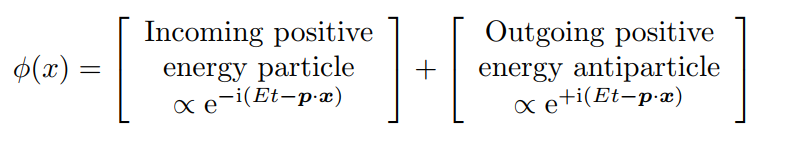
\includegraphics[scale=0.8]{Figures/anti.png}
	\caption{The general solution of the Klei-Gordon equation is a superposition of of positive energy states, only of that of an incoming particle and an outgoing anti-particle}
\end{figure}
We abandon an inherently single-particle description since we have to keep the particles and anti-particles into account.
\section{Field Theories}
A classical field is simply defined as,
\begin{tcolorbox}
A classical field is a piece of mathematical machine that takes a position in spacetime and outputs an object representing the amplitude of the field at that point. The output might be a scalar (in which case we refer to a scalar field), a complex number (a complex scalar field), a vector (in which case we refer to a vector field), a tensor or something more complicated.
\end{tcolorbox}
\subsection{A Massless Scalar Field}
The Lagrangian for a massless salar field $\psi(x)$ is given by,
\begin{equation}
    \mathcal{L}=\frac{1}{2}\partial^\mu\pho\partial_\mu\phi=\frac{1}{2}(\partial_mu\phi)^2
\end{equation}
Where its gradient $\partial_\mu\phi$ is $\partial\phi(x)/\partial x^\mu$. The Lagrangian can also be expanded as,
\begin{equation}
    \mathcal{L}=\frac{1}{2}(\partial_0\phi)^2-\frac{1}{2}\mathbf{\nabla}\phi\cdot\mathbf{\nabla}\phi
\end{equation}
Which neatly resembles $\mathcal{L}=$(kinetic energy)-(potential energy).
\subsection{A Massive Scalar Field}
Including mass in the massless scalar field problem gives us the massive scalar field. In this case, the Lagrangian $\textbf{L}$
also depends on $\phi$, the magnitude of the scalar field along with $\partial_mu\phi$. We do this by introducing a potential energy term $U(\phi)$, and this being proportional to $\phi^2$. Now the Lagrangian can be written as,
\begin{equation}
    \mathcal{L}=\frac{1}{2}(\partial_\mu\phi)^2-\frac{1}{2}m^2\phi^2
\end{equation}
where the $\frac{1}{2}m^2$ factor is to get an interesting result, as we will see below.\\
Using the Lagrangian we obtained, we get the factors,
\begin{equation}
    \frac{\partial L}{\partial\phi}=-m^2\phi
\end{equation}
and,
\begin{equation}
    \frac{\partial L}{\partial(\partial_\mu\phi}=\partial^\mu\phi
\end{equation}
Plugging these into the Euler-Lagrange equation gives us,
\begin{equation}
    (\partial_\mu\partial^\mu+m^2)\phi=0
\end{equation}
We see that the equation of motion of this field theory is the Klein-Gordon equation.
\subsection{An External Source}
Our next step is to introduce interactions into our scalar field. We can do this by introducing a function known as source current $J(x)$, which interacts with the field, giving a potential energy term $-J(x)\phi(x)$. The Lagrangian is written as,
\begin{equation}
    \mathcal{L}=\frac{1}{2}[\partial_\mu\phi(x)]^2-\frac{1}{2}m^2[\phi(x)]^2+J(x)\phi(x)
\end{equation}
And the equations of motion,
\begin{equation}
     (\partial_\mu\partial^\mu+m^2)\phi(x)=J(x)
\end{equation}
\subsection{The $\phi^{4}$ Theory}
To get particles/fields to interact with other particles/fields, we use the $\phi^4$ Lagrangian, where the potential term $U(\phi)$ is proportional to $\phi^4$ instead of $\phi^2$,
\begin{equation}
    \mathcal{L}=\frac{1}{2}\partial^\mu\phi\partial_\mu\phi-\frac{1}{2}m^2\phi^2-\frac{1}{4!}\lambda\phi^4
\end{equation}
which leads to the equation of motion,
\begin{equation}
    (\partial^2+m^2)\phi=-\frac{\lambda}{3!}\phi^3
\end{equation}
Where $\lambda$ is known as the interaction strength. Sadly, this Lagrangian is unsolvable, and we can only use perturbation theory to make predictions out of the $\phi^4$ theory.
\subsection{Two Scalar Fields}
Another method of interacting two particles is by defining two types of particles, described by two fields $\phi_1(x)$ and $\phi_2(x)$. They are said to have the same mass, and interact with themselves and each other via a potential energy $U(\phi_1,\phi_2)=g(\phi^2_1+\phi^2_2)^2$ where $g$ is the interaction strength. The resulting Lagrangian density is given by,
\begin{equation}
    \mathcal{L}=\frac{1}{2}(\partial_\mu\phi_1)^2-\frac{1}{2}(m^2\phi^2_1)+\frac{1}{2}(\partial_\mu\phi_2)^2-\frac{1}{2}(m^2\phi^2_2)-g(\phi^2_1+\phi^2_2)^2
\end{equation}
The above equation shows us the symmetry of the Lagrangian- it does not matter how we define our fields, we still get the same Lagrangian.\\
Transforming the two fields by using the mapping $\phi_1\rightarrow \phi'_1$ and  $\phi_2\rightarrow \phi'_2$, where,
\begin{equation}
    \begin{pmatrix}
    \phi'_1\\
    \phi'_2
    \end{pmatrix}=
    \begin{pmatrix}
    \cos{\theta} & -\sin\theta \\
    \sin\theta & -\cos\theta
    \end{pmatrix}
    \begin{pmatrix}
    \phi_1\\
    \phi_2
    \end{pmatrix}
\end{equation}
then the Lagrangian is still unchanged. We have rotated the fields in $\phi_1-\phi_2$ space. This says that the particles have an internal degree of freedom. The invariance of the physics of the Lagrangian with respect to rotations by $\theta$ in the $\phi_1-\phi_2$ plane expresses an $S0_(2)$ symmetry.
\subsection{The Complex Scalar Field}
A complex field theory can be constructed by making a transformation that simplifies the two scalar fields, by defining two new fields, $\psi$ and $\psi^\dagger$,
\begin{gather}
    \psi=\frac{1}{\sqrt{2}}[\phi_1+i\phi_2]\\
    \psi^\dagger=\frac{1}{\sqrt{2}}[\phi_1-i\phi_2]
\end{gather}
And using the two new fields, we get the Lagrangian,
\begin{equation}
    \mathcal{L}=\partial^\mu\pshi^\dagger\partial_\mu\psi-m^2\psi^\dagger\psi-g(\psi^\dagger\psi)^2
\end{equation}
This is the complex scalar field theory. Although it is made up of two sorts of field, it describes one sort of complex-valued field $\psi$. The Lagrangian is invariant with respect to rotations in the complex plane,
\begin{equation}
    \psi\rightarrow \psi^{i\alpha} \.,\. \psi^{\dagger}\rightarrow e^{-i\alpha}\psi^{\dagger}
\end{equation}
which expresses a $U(1)$ symmetry.